\chapter{The \texttt{ambulance\_game} Python library}
\label{appendix:ambulance_game}

% TODO: Reference sections of thesis throughout
This chapter of the appendix provides an overview of the
\texttt{ambulance\_game} Python library.
This is a library that accompanies all chapters of this thesis and provides
the functionality to run the mathematical models and simulations described
in the thesis.
The library uses the best available tools to ensure the code is correct,
readable, well-documented and properly tested.
These tools are outlined in Section~\ref{sec:intro_test_code}.
The library is also publicly available on GitHub and has been archived on
Zenodo~\cite{ambulance_game_github_repo}.

This appendix chapter is structured based on the Diataxis
framework~\cite{Procida_Diataxis_documentation_framework}.
The structure of the chapter is as follows:

\begin{itemize}
    \item Section~\ref{sec:ambulance_game_installation} provides instructions
        on how to install the library.
    \item Section~\ref{sec:ambulance_game_tutorial} a learning-oriented lesson
        on performing a specific task using the library.
    \item Section~\ref{sec:ambulance_game_how_to} provides a goal-oriented
        how-to guide on how to use the library.
    \item Section~\ref{sec:ambulance_game_reference} provides some technical
        descriptions of the library and how to use it.
    \item Section~\ref{sec:ambulance_game_explanation} provides a discussion
        of some of the details of the library.
\end{itemize}


\section{Installation}\label{sec:ambulance_game_installation}

The \texttt{ambulance\_game} library is published on the Python Package
Index (PyPI)
and can be installed using the \texttt{pip} package manager~\cite{pypi}:

\definecolor{bashcol}{RGB}{211, 211, 211}
\begin{lstlisting}[
    language=bash,
    basicstyle=\ttfamily\scriptsize,
    backgroundcolor=\color{bashcol},
    frame=shadowbox,
    mathescape=false,
]
$ python -m pip install ambulance_game
\end{lstlisting}

Alternatively, a development version of the library can be installed from
GitHub.
The following commands clone the repository, install the \texttt{flit}
package manager and install the library in development mode: 

\begin{lstlisting}[
    language=bash,
    basicstyle=\ttfamily\scriptsize,
    backgroundcolor=\color{bashcol},
    frame=shadowbox,
    mathescape=false,
]
$ git clone https://github.com/MichalisPanayides/AmbulanceDecisionGame.git
$ cd AmbulanceDecisionGame
$ python -m pip install flit
$ python -m flit install --symlink
\end{lstlisting}

To make sure that the library is installed correctly, and to check that the
tests pass, the following command install the \texttt{tox} package manager
and runs the tests:

\begin{lstlisting}[
    language=bash,
    basicstyle=\ttfamily\scriptsize,
    backgroundcolor=\color{bashcol},
    frame=shadowbox,
    mathescape=false,
]
$ python -m pip install tox
$ python -m tox
\end{lstlisting}


\section{Tutorial}\label{sec:ambulance_game_tutorial}

The following tutorial provides the steps to get the Nash
equilibrium of an instance of the game between two hospitals and an ambulance
service provider using the \texttt{ambulance\_game} library.
Table~\ref{tab:ambulance_game_example} provides the parameters of the game
instance.

\begin{table}[H]
    \begin{center}
        \begin{tabular}{||c|c|c|c||}
            \hline
            \(\lambda_2\) & t & \footnotesize{\(\hat{P}\)} & \(\alpha\) \\
            \hline\hline
            8 & 2 & 0.7 & 0.5 \\
            \hline
        \end{tabular}

        \vspace{0.3cm}

        \begin{tabular}{||c|c|c|c|c||}
            \hline
            \(\lambda_1^A\) & \(\mu^A\) & \(C^A\) & \(N^A\) & \(M^A\) \\
            \hline\hline
            1 & 3 & 2 & 10 & 5 \\
            \hline
        \end{tabular}

        \vspace{0.3cm}
        
        \begin{tabular}{||c|c|c|c|c||}
            \hline
            \(\lambda_1^B\) & \(\mu^B\) & \(C^B\) & \(N^B\) & \(M^B\) \\
            \hline\hline
            2 & 1 & 3 & 10 & 5 \\
            \hline
        \end{tabular}
    \end{center}
    \caption{Parameters of the game}
    \label{tab:ambulance_game_example}
\end{table}

A full description of the parameters of the game can also be found in
Section~\ref{sec:game_players_and_parameters}.
The code snippet in Listing~\ref{lst:abg_tutorial_parameters} defines the
parameters of the game instance using Python.

\begin{lstlisting}[
    style=pystyle,
    caption={Python code that defnies the parameters.},
    label={lst:abg_tutorial_parameters},
]
>>> lambda_2 = 8
>>> target = 2
>>> alpha = 0.5
>>> p_hat = 0.7
>>>
>>> lambda_1_1 = 1
>>> mu_1 = 3
>>> num_of_servers_1 = 2
>>> system_capacity_1 = 10
>>> buffer_capacity_1 = 5
>>>
>>> lambda_1_2 = 2
>>> mu_2 = 1
>>> num_of_servers_2 = 3
>>> system_capacity_2 = 10
>>> buffer_capacity_2 = 5

\end{lstlisting}

The arrival rate of type 2 individuals (ambulance patients) is set to
\texttt{lambda\_2 = 8}.
The parameters that correspond to the policy imposed to the hospitals are
\texttt{target = 2} and \texttt{p\_hat = 0.7}.
This means that the hospitals should aim to serve \(70\%\) of the patients
that arrive at the hospital within \(2\) time units.

The python code shown in~\ref{lst:abg_tutorial_game_instance} uses the
parameters of the current game to create matrices \(A\), \(B\) and \(R\)
that represent the payoff matrices of the game and the routing matrix
respectively.
For more information on the matrices of the game, refer to
Section~\ref{sec:queueing_systems_and_normal_form_games}.
The code snippet also uses the \texttt{nashpy} library~\cite{thenashpyproject}
to define the game object.

\begin{lstlisting}[
    style=pystyle,
    caption={Python code that defines the game instance.},
    label={lst:abg_tutorial_game_instance},
]
>>> import ambulance_game as abg
>>> import numpy as np
>>> import nashpy as nash
>>>
>>> A, B, R = abg.game.get_payoff_matrices(
...     lambda_2=lambda_2,
...     target=target,
...     alpha=alpha,
...     p_hat=p_hat,
...     lambda_1_1=lambda_1_1,
...     lambda_1_2=lambda_1_2,
...     mu_1=mu_1,
...     mu_2=mu_2,
...     num_of_servers_1=num_of_servers_1,
...     num_of_servers_2=num_of_servers_2,
...     system_capacity_1=system_capacity_1,
...     system_capacity_2=system_capacity_2,
...     buffer_capacity_1=buffer_capacity_1,
...     buffer_capacity_2=buffer_capacity_2,
... )
>>> game = nash.Game(A, B)

\end{lstlisting}

Thus, a Nash equilibrium of the game can be found using the
\texttt{lemke\_howson} function of the \texttt{nashpy} library.
The Python code shown in Listing~\ref{lst:abg_tutorial_nash_equilibrium}
gets a Nash equilibrium of the game instance.

\begin{lstlisting}[
    style=pystyle,
    caption={Python code that finds a Nash equilibrium of the game instance.},
    label={lst:abg_tutorial_nash_equilibrium},
]
>>> strat_1, strat_2 = game.lemke_howson(initial_dropped_label=0)
>>> strat_1
array([0., 0., 0., 0., 0., 0., 0., 0., 0., 1.])
>>> strat_2
array([0., 0., 0., 0., 0., 1., 0., 0., 0., 0.])

\end{lstlisting}

This corresponds to player \(1\) playing a strategy of
\(\sigma^A = (0, 0, 0, 0, 0, 0, 0, 0, 0, 1)\) and player \(2\) playing a
strategy of \(\sigma^B = (0, 0, 0, 0, 0, 1, 0, 0, 0, 0)\).
This in turn corresponds to player \(1\) choosing a threshold of \(T^A = 10\)
and player \(2\) choosing a threshold of \(T^B = 6\).

Apart from the Nash equilibrium, a learning algorithm can also be used to get
an evolutionary stable strategy (ESS) of the game.
In the code snippet shown in Listing~\ref{lst:abg_tutorial_ard}, the results
of the asymmetric replicator dynamics algorithm run are shown.
The code snippet also uses the \texttt{matplotlib} library to plot the
results of the algorithm.


\definecolor{invisiblecomments}{RGB}{253, 246, 220}
\begin{lstlisting}[
    style=pystyle,
    caption={Python code that runs the asymmetric replicator dynamics algorithm.},
    label={lst:abg_tutorial_ard},
    commentstyle=\color{invisiblecomments},
    showstringspaces=false,
]
>>> import matplotlib.pyplot as plt
>>> xs,ys = game.asymmetric_replicator_dynamics(
...     timepoints=np.linspace(0, 10000, 1000)
... )
>>>
>>> plt.plot(xs[0:30]) # doctest: +SKIP
>>> plt.title("Asymmetric replicator dynamics for player 1") # doctest: +SKIP
>>> plt.xlabel("Timepoints") # doctest: +SKIP
>>> plt.ylabel("Probability") # doctest: +SKIP
>>> plt.show() # doctest: +SKIP
>>>
>>> plt.plot(ys) # doctest: +SKIP
>>> plt.title("Asymmetric replicator dynamics for player 2") # doctest: +SKIP
>>> plt.xlabel("Timepoints") # doctest: +SKIP
>>> plt.ylabel("Probability") # doctest: +SKIP
>>> plt.show() # doctest: +SKIP
    
\end{lstlisting}

\begin{figure}[H]
    \centering
    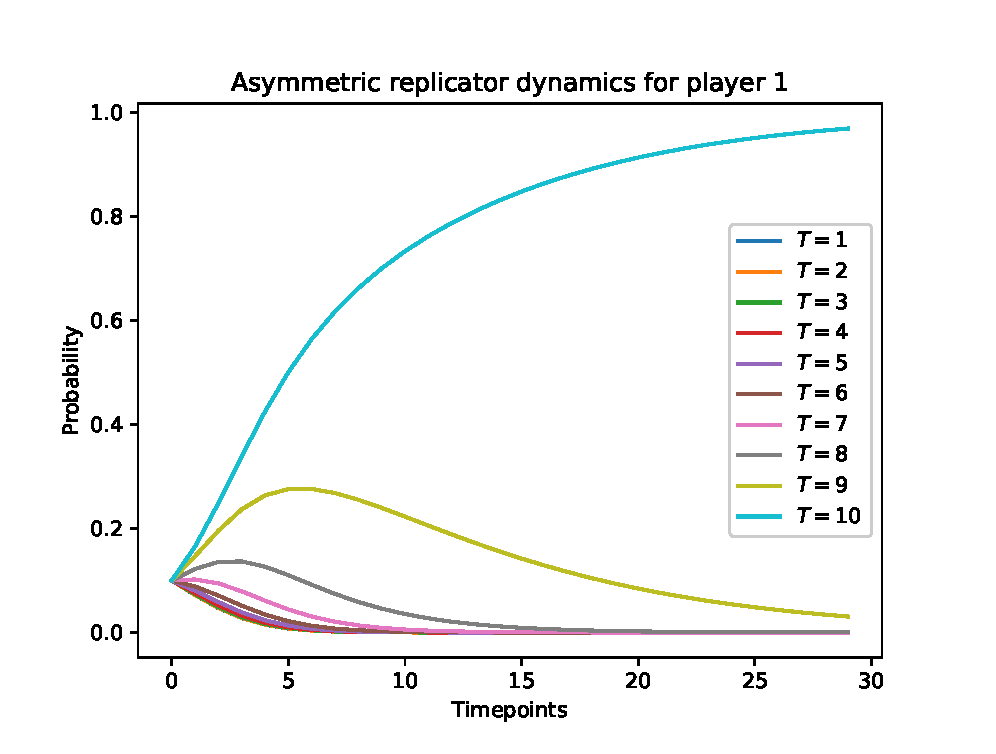
\includegraphics[width=0.49\textwidth]{chapters/00_appendix/01_ambulance_game_library/Bin/ard_p1.eps}
    \includegraphics[width=0.49\textwidth]{chapters/00_appendix/01_ambulance_game_library/Bin/ard_p2.eps}
\end{figure}


From the results of both the Lemke-Howson algorithm and the asymmetric
replicator dynamics algorithm, the same pair of strategies is found.
That is player \(1\) choosing a threshold of \(T^A = 10\) and player \(2\)
choosing a threshold of \(T^B = 6\).
The equivalent strategy of the third player; the ambulance service, can be
found from the routing matrix \(R\) in position \(R_{10, 6}\).


\begin{lstlisting}[
    style=pystyle,
    caption={Python code for the strategy of the third player.},
    label={lst:abg_tutorial_routing_strategy},
]
>>> threshold_1, threshold_2 = 10, 6
>>> prop_A = R[threshold_1 - 1, threshold_2 - 1]
>>> prop_B = 1 - prop_A
>>> np.round(prop_A, 2), np.round(prop_B, 2)
(0.95, 0.05)

\end{lstlisting}

In response to the thresholds chosen by the first two players, the ambulance
service chooses to send \(95\%\) of the ambulances to the first hospital and
\(5\%\) of the ambulances to the second hospital.
Having this percentage of ambulances sent to each hospital, the overall waiting
time of patients at each hospital can be calculated.
The Python code shown in Listing~\ref{lst:abg_tutorial_waiting_time} calculates
the waiting time of patients at each hospital.

\begin{lstlisting}[
    style=pystyle,
    caption={Python code for the waiting time of patients at each hospital.},
    label={lst:abg_tutorial_waiting_time},
]
>>> mean_wait_1 = abg.markov.get_mean_waiting_time_using_markov_state_probabilities(
...     lambda_2=lambda_2 * prop_A,
...     lambda_1=lambda_1_1,
...     mu=mu_1,
...     num_of_servers=num_of_servers_1,
...     threshold=threshold_1,
...     system_capacity=system_capacity_1,
...     buffer_capacity=buffer_capacity_1,
... )
>>> mean_wait_2 = abg.markov.get_mean_waiting_time_using_markov_state_probabilities(
...     lambda_2=lambda_2 * (1 - prop_A),
...     lambda_1=lambda_1_2,
...     mu=mu_2,
...     num_of_servers=num_of_servers_2,
...     threshold=threshold_2,
...     system_capacity=system_capacity_2,
...     buffer_capacity=buffer_capacity_2,
... )
>>> np.round(mean_wait_1, 3)
1.257
>>> np.round(mean_wait_2, 3)
0.632

\end{lstlisting}

The results of the calculations show that the average waiting time of patients
at the first hospital is \(1.257\) time units and the average waiting time of
patients at the second hospital is \(0.632\) time units.
Going back to the parameters that relate to the policy imposed on the hospitals,
\texttt{target = 2} and \texttt{p\_hat = 0.7}.
As stated earlier, that corresponds to both hospitals serving \(70\%\) of the
patients within \(2\) time units.
The mean total time of patients is calculated by adding the average waiting
time and the average service time of patients.

\begin{lstlisting}[
    style=pystyle,
    caption={Python code for the mean total time of patients at each hospital.},
    label={lst:abg_tutorial_mean_total_time},
]
>>> np.round(mean_wait_1 + (1 / mu_1), 3)
1.591
>>> np.round(mean_wait_2 + (1 / mu_2), 3)
1.632
    
\end{lstlisting}

The first mean time in hospital \(1\) for patients is \(1.591\) time units and
the mean time in hospital \(2\) for patients is \(1.632\) time units.


\section{How-to guides}\label{sec:ambulance_game_how_to}

This section contains a series of how-to guides that explain how to use the
library.
This section contains four subsections that explain how to use the library
for the following purposes:

\begin{itemize}
    \item Simulating the hospital using discrete event simulation.
    \item Getting the Markov chain representation of the hospital.
    \item Creating an object oriented implementation of the functionality of
    both the discrete event simulation and the Markov chain representation.
    \item Creating a game theoretic model of the hospital. 
\end{itemize}

\subsection{Discrete Event Simulation}

For the purposes of this study, a discrete event simulation (DES) model was
constructed to support the Markov chain version described in
section~\ref{sec:queueing_section}.
The queueing model was built in python using the Ciw
library~\cite{ciwpython}.

The same performance measures described in Section~\ref{sec:waiting_time},
Section~\ref{sec:blocking_time} and
Section~\ref{sec:proportion_of_individuals_within_time} can also be
calculated using the DES model.
The simulation can be ran a number of times to eliminate stochasticity and the
outcomes of the two methods can be directly comparable.

The DES representation of the hospital network is a discrete event simulation
that is implemented using the \texttt{ciw} library~\cite{ciwpython}.
The required arguments that need to be passed to the
\texttt{simulate\_model} function are the following:

\begin{itemize}
    \item \texttt{lambda\_1} (\(\lambda_1\)): The arrival rate of class 1
    individuals.
    \item \texttt{lambda\_2} (\(\lambda_2\)): The arrival rate of class 2
    individuals.
    \item \texttt{mu} (\(\mu\)): The service rate of the servers.
    \item \texttt{num\_of\_servers} (\(C\)): The number of servers in the
    system.
    \item \texttt{threshold} (\(T\)): The threshold that indicates when to start
    blocking type 2 individuals.
\end{itemize}

\begin{lstlisting}[style=pystyle]
>>> lambda_1 = 3
>>> lambda_2 = 2
>>> mu = 1
>>> num_of_servers = 6
>>> threshold = 10
    
\end{lstlisting}

To get the \texttt{simulation} object with all the data records, the following
code can be used:

\begin{lstlisting}[style=pystyle]
>>> import ambulance_game as abg
>>> import numpy as np
>>> simulation = abg.simulation.simulate_model(
...     lambda_1=lambda_1,
...     lambda_2=lambda_2,
...     mu=mu,
...     num_of_servers=num_of_servers,
...     threshold=threshold,
...     seed_num=0,
... )
>>> simulation.get_all_records()[4]
Record(id_number=2, customer_class=0, node=2, arrival_date=0.5727571550618586, waiting_time=0.0, service_start_date=0.5727571550618586, service_time=0.7159547497671506, service_end_date=1.2887119048290092, time_blocked=0.0, exit_date=1.2887119048290092, destination=-1, queue_size_at_arrival=1, queue_size_at_departure=3)

\end{lstlisting}

Additional arguments that can be passed to the function are:
\begin{itemize}
    \item \texttt{system\_capacity} (\(N\)): The maximum number of individuals
    in waiting zone 1.
    \item \texttt{buffer\_capacity} \(M\): The maximum number of individuals in
    waiting zone 2.
    \item \texttt{seed\_num}: The seed number for the random number generator.
    \item \texttt{runtime}: How long to run the simulation for.
\end{itemize}

From a single run of the simulation the data records can be used to get the
average for certain performance measures.
The following code can be used to get the mean waiting time, blocking time,
service time and the proportion of individuals within target.

\begin{lstlisting}[style=pystyle]
>>> records = simulation.get_all_records()
>>> mean_wait = np.mean(
...     [w.waiting_time for w in records]
... )
>>> mean_wait
0.23845862661827116

>>> mean_block = np.mean(
...     [b.time_blocked for b in records]
... )
>>> mean_block
0.08501727452006658

>>> mean_service = np.mean(
...     [s.service_time for s in records]
... )
>>> mean_service
0.7102610863960119

>>> target = 1
>>> proportion_within_target = np.mean(
...     [r.waiting_time + r.service_time <= target for r in records]
... )
>>> proportion_within_target
0.6200119712689545

\end{lstlisting}

To reduce the effects of stochasticity in the simulation, the simulation can be
run numerous times and get the average performance measures out of all the runs.

\begin{lstlisting}[style=pystyle]
>>> all_simulations = abg.simulation.get_multiple_runs_results(
...     lambda_1=lambda_1,
...     lambda_2=lambda_2,
...     mu=mu,
...     num_of_servers=num_of_servers,
...     threshold=threshold,
...     system_capacity=20,
...     buffer_capacity=10,
...     seed_num=0,
...     runtime=2000,
...     num_of_trials=10,
...     target=1,
... )
>>> mean_wait = np.mean([
...     np.mean(w.waiting_times) for w in all_simulations
... ])
>>> mean_wait
0.35585979549204577

>>> mean_service = np.mean([
...     np.mean(s.service_times) for s in all_simulations
... ])
>>> mean_service
1.002184850213415

>>> mean_block = np.mean([
...     np.mean(b.blocking_times) for b in all_simulations
... ])
>>> mean_block
0.3976966024549059

>>> mean_prop = np.mean([
...     p.proportion_within_target for p in all_simulations
... ])
>>> mean_prop
0.45785790578122043

\end{lstlisting}

To get the steady state probabilities of the model based on the simulation the
following code can be used:

\begin{lstlisting}[style=pystyle]
>>> import numpy as np
>>> import ambulance_game as abg
>>> simulation_object = abg.simulation.simulate_model(
...     lambda_1=1,
...     lambda_2=2,
...     mu=2,
...     num_of_servers=2,
...     threshold=3,
...     system_capacity=4,
...     buffer_capacity=2,
...     seed_num=0,
...     runtime=2000,
... )
>>> probs = abg.simulation.get_simulated_state_probabilities(
...    simulation_object=simulation_object,
... )
>>> np.round(probs, decimals=3)
array([[0.166, 0.266, 0.192, 0.147, 0.025],
       [  nan,   nan,   nan, 0.094, 0.024],
       [  nan,   nan,   nan, 0.058, 0.027]])

>>> total = np.nansum(probs)
>>> np.round(total, decimals=5)
1.0

\end{lstlisting}

Similarly to get the average steady state probabilities over multiple runs,
one can use the code in Listing~\ref{lst:average_simulated_state_probabilities}
to get the average steady state probabilities out of multiple runs.

\begin{lstlisting}[
    style=pystyle,
    caption={The average steady state probabilities of the model based on the simulation.},
    label={lst:average_simulated_state_probabilities}
]
>>> import numpy as np
>>> import ambulance_game as abg
>>> probs = abg.simulation.get_average_simulated_state_probabilities(
...     lambda_1=1,
...     lambda_2=2,
...     mu=2,
...     num_of_servers=2,
...     threshold=3,
...     system_capacity=4,
...     buffer_capacity=2,
...     seed_num=0,
...     runtime=2000,
...     num_of_trials=10,
... )
>>> np.round(probs, decimals=3)
array([[0.18 , 0.267, 0.197, 0.144, 0.024],
       [  nan,   nan,   nan, 0.085, 0.022],
       [  nan,   nan,   nan, 0.054, 0.026]])

>>> total = np.nansum(probs)
>>> np.round(total, decimals=5)
1.0

\end{lstlisting}

As an additional feature, the simulation can use a service rate that is state
dependent, server dependent or both.
This feature was implemented to accompany
Chapter~\ref{sec:agent_based_extension} of this thesis.
The state-dependent service rate is defined as a dictionary with the keys
being the states.
The server-dependent service rate is defined as a dictionary with the keys
being the servers.
The state and server dependent service rate is defined as a dictionary with
the keys being the servers and the values being dictionaries with the keys
being the states.
The code snippet in Listing~\ref{lst:state_server_dependent_service_rate} shows
examples of how to define these service rates.

\begin{lstlisting}[
    style=pystyle,
    caption={Examples of how to define the state-dependent, server-dependent and state and server dependent service rates.},
    label={lst:state_server_dependent_service_rate}
]
>>> state_dependent_service_rate = {
...     (0, 0): np.nan,
...     (0, 1): 0.5,
...     (0, 2): 0.3,
...     (0, 3): 0.2,
...     (1, 3): 0.2,
...     (0, 4): 0.2,
...     (1, 4): 0.4,
... }
>>> server_dependent_service_rate = {
...     1: 0.5,
...     2: 0.3,
... }
>>> state_server_dependent_service_rate = {
...     1: {
...         (0, 1): 0.5,
...         (0, 2): 0.3,
...         (0, 3): 0.2,
...         (1, 3): 0.2,
...         (0, 4): 0.2,
...         (1, 4): 0.4,
...     },
...     2: {
...         (0, 1): 1.5,
...         (0, 2): 1.3,
...         (0, 3): 1.2,
...         (1, 3): 1.2,
...         (0, 4): 1.2,
...         (1, 4): 1.4,
...     },
... }

\end{lstlisting}

Note that for this particular example server \(1\) is much slower than server
\(2\) for all states.
The code shown in~\ref{lst:state_server_dependent_service_rate_simulation}
shows how to use the state and server dependent service rate in the simulation.
At the end the busy time of the two servers can be compared.

\begin{lstlisting}[
    style=pystyle,
    caption={The simulation using the state and server dependent service rate.},
    label={lst:state_server_dependent_service_rate_simulation}
]
>>> simulation_object = abg.simulation.simulate_model(
...     lambda_1=0.2,
...     lambda_2=0.15,
...     mu=state_server_dependent_service_rate,
...     num_of_servers=2,
...     threshold=4,
...     seed_num=0,
...     runtime=100,
... )
>>> servers = simulation_object.nodes[2].servers
>>> [server.busy_time for server in servers]
[32.88159812544271, 8.576662185652019]

\end{lstlisting}

It can be seen that the busy time of server \(1\) is much higher than the busy
time of server \(2\).


\subsection{Markov Chains}

This subsection presents a guide on how to use the \texttt{ambulance\_game}
library to create and solve the Markov chain (MC) model of the hospital network
discussed in this thesis (see Chapter~\ref{sec:queueing_section}).
The parameters used are defined in Listing~\ref{lst:abg_how_to_markov}.
For more information on the parameters, refer to
Section~\ref{sec:queueing_section}.


\begin{lstlisting}[
    style=pystyle,
    caption={Python code for the parameters used in the Markov chain model.},
    label={lst:abg_how_to_markov},
]
>>> lambda_1 = 1
>>> lambda_2 = 2
>>> mu = 5
>>>
>>> num_of_servers = 1
>>> threshold = 2
>>> system_capacity = 3
>>> buffer_capacity = 1

\end{lstlisting}

This section focuses on the $\texttt{markov}$ module of the ambulance\_game
library which focuses on the Markov model.
Function \texttt{build\_states} takes in the \texttt{threshold}, the
\texttt{system\_capacity} and the \texttt{buffer\_capacity} variables and
returns a list of all the states of the MC model.

\begin{lstlisting}[
    style=pystyle,
    caption={Python code for building the states of the Markov chain model.},
    label={lst:abg_how_to_markov_states},
]
>>> import ambulance_game as abg
>>> all_states = abg.markov.build_states(
...     threshold=threshold,
...     system_capacity=system_capacity,
...     buffer_capacity=buffer_capacity,
... )
>>> all_states
[(0, 0), (0, 1), (0, 2), (1, 2), (0, 3), (1, 3)]

\end{lstlisting}

To visualise the list of states that are returned by the
\texttt{build\_states} function, the \texttt{visualise\_markov\_chain}
function can be used.

\definecolor{invisiblecomments}{RGB}{253, 246, 220}
\begin{lstlisting}[
    style=pystyle,
    caption={Python code for visualising the Markov chain model.},
    label={lst:abg_how_to_markov_visualise},
    commentstyle=\color{invisiblecomments},
]
>>> abg.markov.visualise_markov_chain(
...     num_of_servers=num_of_servers,
...     threshold=threshold,
...     system_capacity=system_capacity,
...     buffer_capacity=buffer_capacity,
... ) # doctest: +SKIP
\end{lstlisting}

\begin{figure}[H]
    \centering
    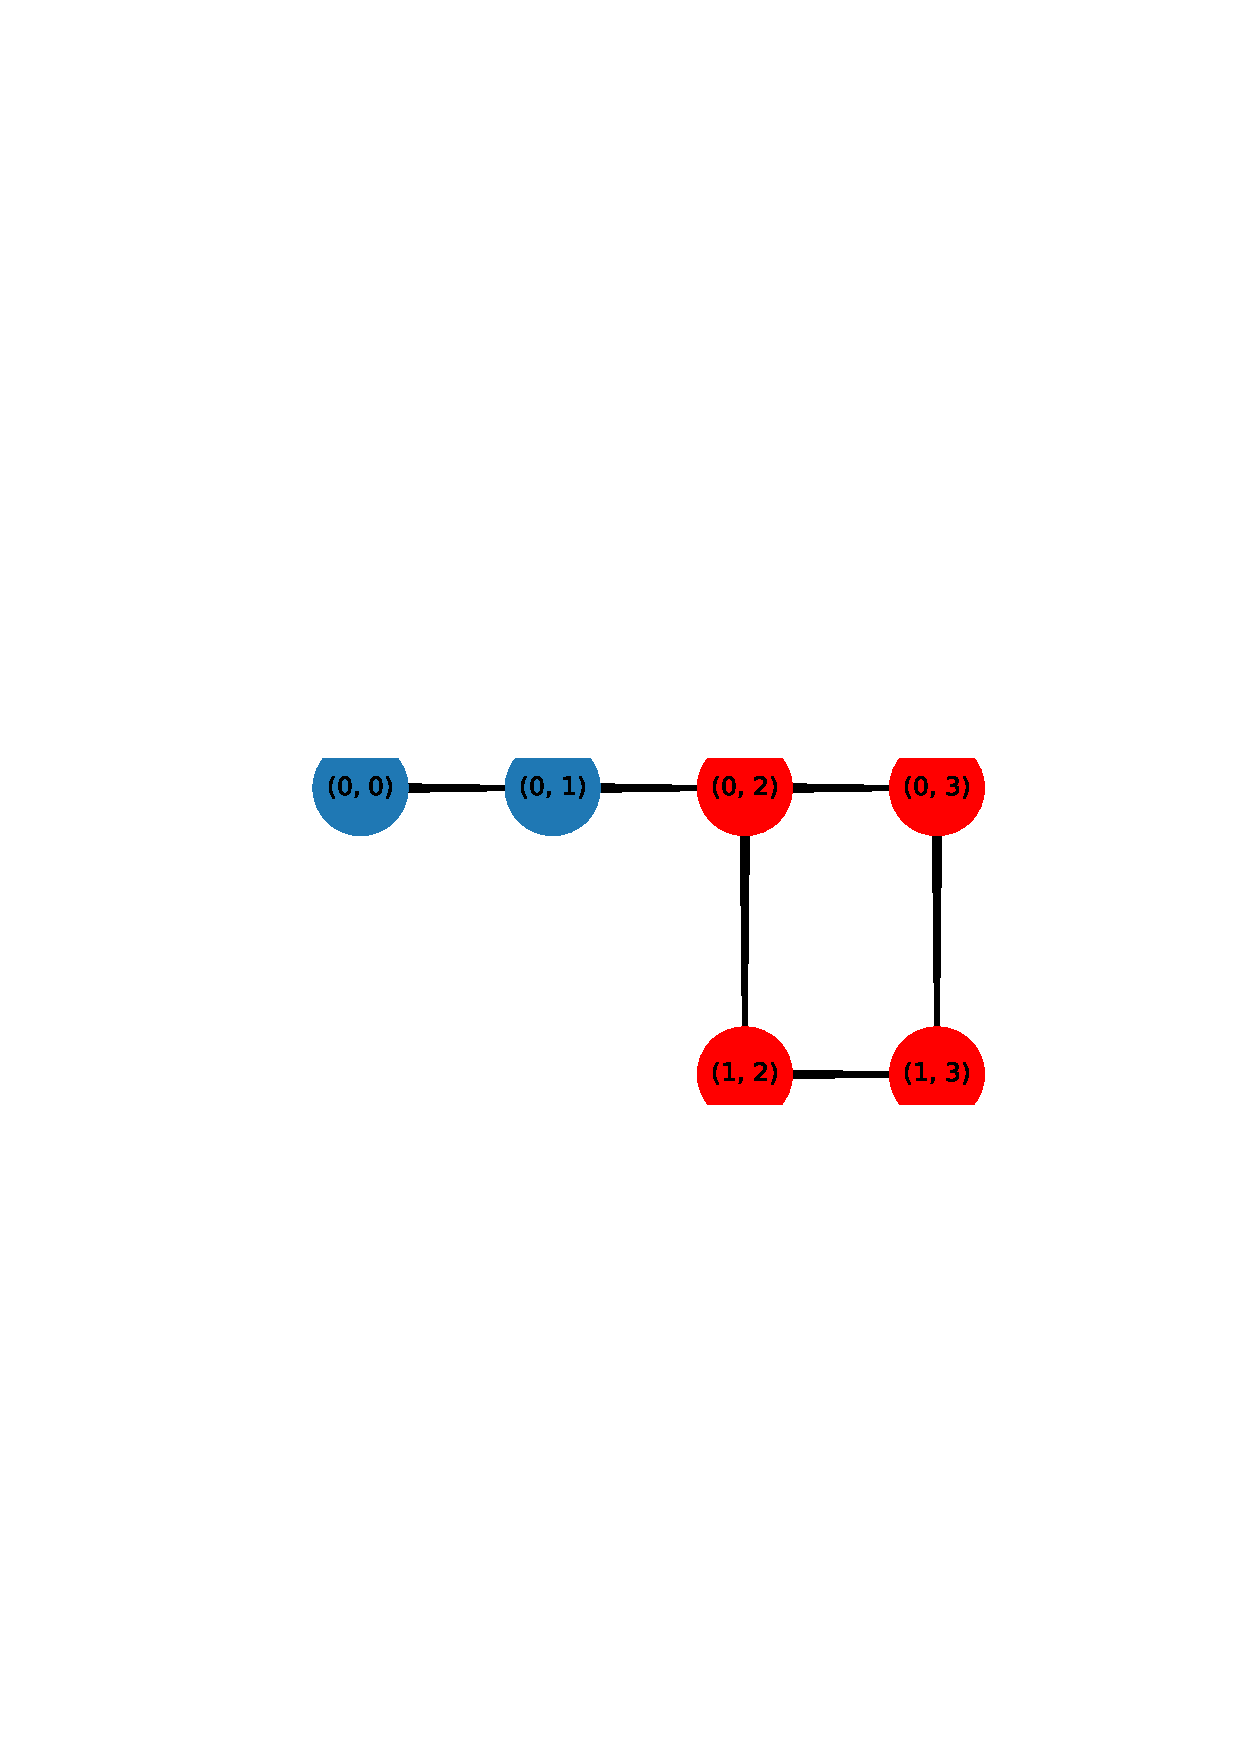
\includegraphics[width=\textwidth]{chapters/00_appendix/01_ambulance_game_library/Bin/visualise_markov.pdf}
    
\end{figure}

The function \texttt{get\_transition\_matrix} builds the transition matrix
of the MC model.

\begin{lstlisting}[
    style=pystyle,
    caption={Python code for building the transition matrix of the Markov
    chain model.},
    label={lst:abg_how_to_markov_transition},
]
>>> Q = abg.markov.get_transition_matrix(
...     lambda_1=lambda_1,
...     lambda_2=lambda_2,
...     mu=mu,
...     num_of_servers=num_of_servers,
...     threshold=threshold,
...     system_capacity=system_capacity,
...     buffer_capacity=buffer_capacity,
... )
>>> Q
array([[-3.,  3.,  0.,  0.,  0.,  0.],
       [ 5., -8.,  3.,  0.,  0.,  0.],
       [ 0.,  5., -8.,  2.,  1.,  0.],
       [ 0.,  0.,  5., -6.,  0.,  1.],
       [ 0.,  0.,  5.,  0., -7.,  2.],
       [ 0.,  0.,  0.,  5.,  0., -5.]])

\end{lstlisting}

The functions shown in Listing~\ref{lst:abg_how_to_markov_steady_state} can be
used to calculate the steady state probabilities of the MC model.
The steady state probabilities can be calculated using a numerical method or
an algebraic method.
For more information on the methods, refer to
Section~\ref{sec:ambulance_game_explanation}.

\begin{lstlisting}[
    style=pystyle,
    caption={Python code for building the steady state probabilities of the
    Markov chain model.},
    label={lst:abg_how_to_markov_steady_state},
]
>>> pi = abg.markov.get_steady_state_numerically(Q)
>>> pi
array([0.44853393, 0.26912036, 0.16147222, 0.07381587, 0.02306746,
       0.02399016])

>>> pi = abg.markov.get_steady_state_algebraically(Q)
>>> pi
array([0.44853393, 0.26912036, 0.16147222, 0.07381587, 0.02306746,
       0.02399016])
    
\end{lstlisting}

The functions shown in Listing~\ref{lst:abg_how_to_markov_expected_number}
can be used to calculate the expected number of patients in the system,
service area and buffer centre.

\begin{lstlisting}[
    style=pystyle,
    caption={Python code for getting the expected number of patients in the
    Markov chain model.},
    label={lst:abg_how_to_markov_expected_number},
]
>>> import numpy as np
>>> np.round(
...     abg.markov.get_mean_number_of_individuals_in_system(
...         pi=pi, states=all_states
...     ), 3
... )
0.979

>>> np.round(
...     abg.markov.get_mean_number_of_individuals_in_service_area(
...         pi=pi, states=all_states
...     ), 3
... )
0.881

>>> np.round(
...     abg.markov.get_mean_number_of_individuals_in_buffer_center(
...         pi=pi, states=all_states
...     ), 3
... )
0.098

\end{lstlisting}

To get the mean waiting time of patients in the system, the code snippet
shown in Listing~\ref{lst:abg_how_to_markov_waiting} can be used.

\begin{lstlisting}[
    style=pystyle,
    caption={Python code for getting the expected waiting time of individuals
    in the Markov chain model.},
    label={lst:abg_how_to_markov_waiting},
]
>>> np.round(
...     abg.markov.get_mean_waiting_time_using_markov_state_probabilities(
...         lambda_1=lambda_1,
...         lambda_2=lambda_2,
...         mu=mu,
...         num_of_servers=num_of_servers,
...         threshold=threshold,
...         system_capacity=system_capacity,
...         buffer_capacity=buffer_capacity,
...     ), 4
... )
0.1195

\end{lstlisting}

Note that an additional argument \texttt{class_type} can be used to get the
mean waiting time of type 1 or type 2 individuals that takes values \(0\) and
\(1\), respectively.
The default value of \texttt{class_type} is set to \texttt{None} which
returns the mean waiting time of all individuals.

To get the mean blocking time of type 2 patients in the system (ambulance
patients), the code snippet shown in
Listing~\ref{lst:abg_how_to_markov_blocking} can be used.

\begin{lstlisting}[
    style=pystyle,
    caption={Python code for getting the expected blocking time of type 2
    individuals in the Markov chain model.},
    label={lst:abg_how_to_markov_blocking},
]
>>> np.round(
...     abg.markov.get_mean_blocking_time_using_markov_state_probabilities(
...         lambda_1=lambda_1,
...         lambda_2=lambda_2,
...         mu=mu,
...         num_of_servers=num_of_servers,
...         threshold=threshold,
...         system_capacity=system_capacity,
...         buffer_capacity=buffer_capacity,
...     ), 4
... )
0.0542

\end{lstlisting}

To get the proportion of individuals that are seen within a time target, the
code snippet shown in Listing~\ref{lst:abg_how_to_markov_proportion} can be
used.

\begin{lstlisting}[
    style=pystyle,
    caption={Python code for getting the proportion of individuals within
    target using the Markov chain model.},
    label={lst:abg_how_to_markov_proportion},
]
>>> np.round(
...     abg.markov.proportion_within_target_using_markov_state_probabilities(
...         lambda_1=lambda_1,
...         lambda_2=lambda_2,
...         mu=mu,
...         num_of_servers=num_of_servers,
...         threshold=threshold,
...         system_capacity=system_capacity,
...         buffer_capacity=buffer_capacity,
...         class_type=None,
...         target=0.5,
...     ), 3
... )
0.791

\end{lstlisting}


\subsection{Object Oriented Implementation} % Should this be here?


\input{chapters/00_appendix/01_ambulance_game_library/03_how_to_guides/04_game.tex}



\section{Reference}\label{sec:ambulance_game_reference}

The \texttt{ambulance\_game} library is structured as shown in
Figure~\ref{fig:ambulance_game_structure}.

\begin{figure}[H]
    \dirtree{%
        .1 ambulance\_game.
        .2 markov/.
        .3 \_\_init\_\_.py.
        .3 blocking.py.
        .3 graphical.py. 
        .3 markov.py. 
        .3 proportion.py. 
        .3 tikz.py. 
        .3 utils.py. 
        .3 waiting.py.
        .2 simulation.
        .3 \_\_init\_\_.py.
        .3 dists.py.
        .3 simulation.py.
        .2 comparisons.py.
        .2 game.py.
        .2 queue.py.
    }
    \caption{Structure of the modules in the \texttt{ambulance\_game} library}
    \label{fig:ambulance_game_structure}
\end{figure}


Below is a list of all the functions in the \texttt{ambulance\_game} library
sorted by the modules they are in.
The entries that start with a capital letter are classes and the rest are
functions.

\scriptsize
\begin{itemize}
    \item \texttt{blocking.py}
    \begin{itemize}
        \item \texttt{get\_coefficients\_row\_of\_array\_associated\_with\_state}
        \item \texttt{get\_blocking\_time\_linear\_system}
        \item \texttt{convert\_solution\_to\_correct\_array\_format}
        \item \texttt{get\_blocking\_times\_of\_all\_states\_using\_direct\_approach}
        \item \texttt{mean\_blocking\_time\_formula\_using\_direct\_approach}
        \item \texttt{mean\_blocking\_time\_formula\_using\_closed\_form\_approach}
        \item \texttt{get\_mean\_blocking\_time\_using\_markov\_state\_probabilities}
        \item \texttt{get\_mean\_blocking\_difference\_using\_markov}
    \end{itemize}
    \item \texttt{graphical.py}
    \begin{itemize}
        \item \texttt{reset\_L\_and\_R\_in\_array}
        \item \texttt{find\_next\_permutation\_over}
        \item \texttt{find\_next\_permutation\_over\_L\_and\_R}
        \item \texttt{generate\_next\_permutation\_of\_edges}
        \item \texttt{check\_permutation\_is\_valid}
        \item \texttt{get\_rate\_of\_state\_00\_graphically}
        \item \texttt{get\_all\_permutations}
        \item \texttt{get\_permutations\_ending\_in\_R}
        \item \texttt{get\_permutations\_ending\_in\_D\_where\_any\_RL\_exists}
        \item \texttt{get\_permutations\_ending\_in\_L\_where\_any\_RL\_exists}
        \item \texttt{get\_permutations\_ending\_in\_RL\_where\_RL\_exists\_only\_at\_the\_end}
        \item \texttt{get\_coefficient}
    \end{itemize}
    \item \texttt{markov.py}
    \begin{itemize}
        \item \texttt{build\_states}
        \item \texttt{visualise\_markov\_chain}
        \item \texttt{get\_transition\_matrix\_entry}
        \item \texttt{get\_symbolic\_transition\_matrix}
        \item \texttt{get\_transition\_matrix\_by\_iterating\_through\_all\_entries}
        \item \texttt{get\_all\_pairs\_of\_states\_with\_non\_zero\_entries}
        \item \texttt{state\_after\_threshold}
        \item \texttt{state\_before\_threshold}
        \item \texttt{state\_at\_threshold}
        \item \texttt{get\_transition\_matrix}
        \item \texttt{convert\_symbolic\_transition\_matrix}
        \item \texttt{is\_steady\_state}
        \item \texttt{get\_steady\_state\_numerically}
        \item \texttt{get\_steady\_state\_algebraically}
        \item \texttt{get\_markov\_state\_probabilities}
        \item \texttt{get\_mean\_number\_of\_individuals\_in\_system}
        \item \texttt{get\_mean\_number\_of\_individuals\_in\_service\_area}
        \item \texttt{get\_mean\_number\_of\_individuals\_in\_buffer\_center}
    \end{itemize}
    \item \texttt{proportion.py}
    \begin{itemize}
        \item \texttt{product\_of\_all\_elements}
        \item \texttt{general\_psi\_function}
        \item \texttt{specific\_psi\_function}
        \item \texttt{hypoexponential\_cdf}
        \item \texttt{erlang\_cdf}
        \item \texttt{get\_probability\_of\_waiting\_time\_in\_system\_less\_than\_target\_for\_state}
        \item \texttt{get\_proportion\_of\_individuals\_within\_time\_target}
        \item \texttt{overall\_proportion\_of\_individuals\_within\_time\_target}
        \item \texttt{proportion\_within\_target\_using\_markov\_state\_probabilities}
    \end{itemize}
    \item \texttt{tikz.py}
    \begin{itemize}
        \item \texttt{generate\_code\_for\_tikz\_figure}
        \item \texttt{build\_body\_of\_tikz\_spanning\_tree}
        \item \texttt{get\_tikz\_code\_for\_permutation}
        \item \texttt{generate\_code\_for\_tikz\_spanning\_trees\_rooted\_at\_00}
    \end{itemize}
    \item \texttt{utils.py}
    \begin{itemize}
        \item \texttt{is\_waiting\_state}
        \item \texttt{is\_blocking\_state}
        \item \texttt{is\_accepting\_state}
        \item \texttt{expected\_time\_in\_markov\_state\_ignoring\_arrivals}
        \item \texttt{expected\_time\_in\_markov\_state\_ignoring\_class\_2\_arrivals}
        \item \texttt{prob\_service}
        \item \texttt{prob\_class\_1\_arrival}
        \item \texttt{get\_probability\_of\_accepting}
        \item \texttt{get\_proportion\_of\_individuals\_not\_lost}
        \item \texttt{get\_accepting\_proportion\_of\_class\_2\_individuals}
        \item \texttt{get\_accepting\_proportion\_of\_individuals}
    \end{itemize}
    \item \texttt{waiting.py}
    \begin{itemize}
        \item \texttt{get\_waiting\_time\_for\_each\_state\_recursively}
        \item \texttt{mean\_waiting\_time\_formula\_using\_recursive\_approach}
        \item \texttt{get\_coefficients\_row\_of\_array\_for\_state}
        \item \texttt{get\_waiting\_time\_linear\_system}
        \item \texttt{convert\_solution\_to\_correct\_array\_format}
        \item \texttt{get\_waiting\_times\_of\_all\_states\_using\_direct\_approach}
        \item \texttt{mean\_waiting\_time\_formula\_using\_direct\_approach}
        \item \texttt{mean\_waiting\_time\_formula\_using\_closed\_form\_approach}
        \item \texttt{overall\_waiting\_time\_formula}
        \item \texttt{get\_mean\_waiting\_time\_using\_markov\_state\_probabilities}
    \end{itemize}
    \item \texttt{simulation.py}
    \begin{itemize}
        \item \texttt{build\_model}
        \item \texttt{build\_custom\_node}
        \item \texttt{simulate\_model}
        \item \texttt{extract\_times\_from\_records}
        \item \texttt{extract\_times\_from\_individuals}
        \item \texttt{get\_list\_of\_results}
        \item \texttt{get\_multiple\_runs\_results}
        \item \texttt{extract\_total\_individuals\_and\_the\_ones\_within\_target\_for\_both\_classes}
        \item \texttt{get\_mean\_proportion\_of\_individuals\_within\_target\_for\_multiple\_runs}
        \item \texttt{get\_simulated\_state\_probabilities}
        \item \texttt{get\_average\_simulated\_state\_probabilities}
        \item \texttt{get\_mean\_blocking\_difference\_between\_two\_systems}
    \end{itemize}
    \item \texttt{dists.py}
    \begin{itemize}
        \item \texttt{StateDependentExponential}
        \item \texttt{ServerDependentExponential}
        \item \texttt{StateServerDependentExponential}
        \item \texttt{is\_state\_dependent}
        \item \texttt{is\_server\_dependent}
        \item \texttt{is\_state\_server\_dependent}
        \item \texttt{get\_service\_distribution}
        \item \texttt{get\_arrival\_distribution}
    \end{itemize}
    \item \texttt{comparisons.py}
        \item \texttt{get\_heatmaps}
        \item \texttt{get\_mean\_waiting\_time\_from\_simulation\_state\_probabilities}
        \item \texttt{get\_mean\_blocking\_time\_from\_simulation\_state\_probabilities}
        \item \texttt{get\_proportion\_within\_target\_from\_simulation\_state\_probabilities}
        \item \texttt{get\_waiting\_time\_comparisons}
        \item \texttt{get\_blocking\_time\_comparisons}
        \item \texttt{get\_proportion\_comparison}
        \item \texttt{get\_simulation\_and\_markov\_outputs}
        \item \texttt{plot\_output\_comparisons}
    \item \texttt{game.py}
    \begin{itemize}
        \item \texttt{calculate\_class\_2\_individuals\_best\_response}
        \item \texttt{get\_routing\_matrix}
        \item \texttt{get\_individual\_entries\_of\_matrices}
        \item \texttt{compute\_tasks}
        \item \texttt{build\_matrices\_from\_computed\_tasks}
        \item \texttt{get\_payoff\_matrices}
        \item \texttt{build\_game\_using\_payoff\_matrices}
    \end{itemize}
    \item \texttt{queue.py}
    \begin{itemize}
        \item \texttt{Queue}
    \end{itemize}
\end{itemize}
\normalsize


\section{Explanation}\label{sec:ambulance_game_explanation}

% - graphical.py?
% - Nashpy and ciw
% - np.linalg.solve, np.linalg.lstsq, sci.integrate.odeint, sci.integrate.solve_ivp
% - sci.optimize.brentq
% - In-depth explanation of the functionality of some code
%     - get_transition_matrix VS get_transition_matrix_by_iterating_through_all_entries
%     - get_symbolic_transition_matrix
%     - is_steady_state
%     - graphical.py module
%     - psi_func, specific_psi_func
%     - 
